\chapter{\ifenglish Background Knowledge and Theory\else ทฤษฎีที่เกี่ยวข้อง\fi}

การทำโครงงาน เริ่มต้นด้วยการศึกษาค้นคว้า ทฤษฎีที่เกี่ยวข้อง หรือ งานวิจัย/โครงงาน ที่เคยมีผู้นำเสนอไว้แล้ว ซึ่งเนื้อหาในบทนี้ก็จะเกี่ยวกับการอธิบายถึงสิ่งที่เกี่ยวข้องกับโครงงาน 
เพื่อให้ผู้อ่านเข้าใจเนื้อหาในบทถัดไปได้ง่ายขึ้น เนื้อหาในบทนี้จะแบ่งออกเป็นดังนี้

\section{MediaPipe Holistic}
อัลกอริทึมในการตรวจจับการเคลื่อนไหวของท่าทาง ใบหน้า และมือได้แบบเรียลไทม์ และสามารถที่จะรองรับอุปกรณ์
ทำให้เป็นวิธีการตรวจจับใบหน้าที่มีประสิทธิภาพ จุดเด่นหลักของ MediaPipe คือความรวดเร็วของการประมวลผลรูปภาพแบบเรียลไทม์
ซึ่งการใช้งานส่วนใหญ่นิยมใช้กับ OpenCV ที่ใช้ภาษาไพธอน (Python) \cite{Mediapipe} โดยแอปพลิเคชันที่ MediaPipe สามารถทำได้มีดังนี้
\begin{enumerate}
  \item การตราจจับใบหน้า
  \item การตราจจับท่วงท่า
  \item การตราจจับสิ่งของ
  \item การตรวจจับเส้นผมบนหัว
  \item การตรวจจับท่าทางของมือ
\end{enumerate}
ซึ่งในโครงงานนี้เลือกที่จะเอาการตรวจจับใบหน้ามาใช้งาน

\section{RESTful API}
เป็นแนวทางในการสร้างเว็บเซอร์วิส (Web Service) โดยเรียกใช้ผ่านทางเมท็อด GET POST PUT และ DELETE
โดย RESTful จะอยู่บนพื้นฐานของเกณฑ์วิธีขนส่งข้อความหลายมิติ (Hypertext Transfer Protocol: HTTP) โดยผู้รับบริการ (Client) จะส่ง
คำขอ (Request) ไปยังรหัสสืบค้นข้อมูลซึ่งระบุแหล่งที่อยู่ของทรัพยากรที่ต้องการ (Uniform Resource Locator: URI) ที่กำหนด และรับ Response กลับมาเป็น Payload 
ในรูปแบบของ (HyperText Markup Language: HTML), (Document Markup Language: XML), (JavaScript Object Notation: JSON) หรือรูปแบบ (format) อื่น ๆ \cite{REST}
ซึ่งในโครงงานนี้จะใช้ Payload แบบ JSON โดย RESTful API จะประกอบไปด้วย
\begin{itemize}
  \item Client - ผู้ที่เข้ามาเป็น Request resource
  \item Server - ผู้ที่ให้บริการ Resource
\end{itemize}
\cleardoublepage


\begin{figure}[!ht]
  \begin{center}
    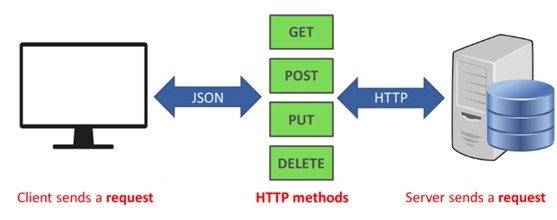
\includegraphics[scale=.6]{pic/restapi.jpg}
    \caption[ผังการทำงานของ RESTful]{ผังการทำงานของ RESTful}
    \label{fig:restapi}
  \end{center}
\end{figure}

\section{Image Processing }
เป็นกระบวนการจัดการและวิเคราะห์รูปภาพให้เป็นข้อมูลในแบบดิจิทัล โดยใช้คอมพิวเตอร์ 
เพื่อให้ได้ข้อมูลที่เราต้องการทั้งในเชิงคุณภาพและปริมาณ (ขนาด รูปร่าง) \cite{Image} โดยกระบวนการจัดการและวิเคราะห์รูปภาพที่ใช้ในโครงงานนี้ มีดังนี้

\subsection{การปรับปรุงคุณภาพของภาพ   (Image Enhancement and Restoration) }
การปรับปรุงคุณภาพของภาพเป็นการปรับปรุงหรือซ่อมแซมให้ข้อมูลภาพที่มีอยู่นั้นมี คุณภาพดีขึ้น เช่น ภาพที่ได้มาอาจมีความคมชัด (Contrast) น้อยหรือเบลอ ไม่คมชัด 
เราสามารถปรับภาพให้คมชัดได้ด้วยเทคนิค เช่น การปรับค่าความคมชัด (Contrast Enhancement) หรือการปรับเน้นเส้นขอบภาพ (Edge Enhancement) 
หรือในกรณีที่ภาพที่มี อยู่มีความไม่สมบูรณ์ เช่น มีสัญญาณรบกวน (Noise) เราสามารถใช้เทคนิคการกรองสัญญาณ ภาพ (Image Filtering) เพื่อกำจัดสัญญาณรบกวนได้

\subsection{การบีบอัดข้อมูลภาพ (Image compression)}
\begin{enumerate}
  \item \textbf{การบีบอัดแบบไม่มีการสูญเสียรายละเอียดข้อมูล (Lossless compression)} \\
  ค่าความสว่างของแต่ละจุดภาพจะยังคงอยู่เหมือนเดิมทุกประการ หรือไม่มีการเปลี่ยนแปลงค่าของแต่ละจุดภาพ 
  ซึ่งการบีบอัดวิธีนี้จะอาศัยเทคนิคการจัดเก็บข้อมูลเชิงเลขในการลดขนาดของข้อมูล
  \item \textbf{การบีบอัดแบบสูญเสียรายละเอียดข้อมูล (Lossy compression)} \\
  วิธีการนี้จะมีการเปลี่ยนแปลงค่าความสว่างของจุดภาพนั่นหมายความว่า วิธีการนี้ไม่เหมาะสมสำหรับข้อมูลภาพที่ต้องมีการจำแนกข้อมูล (Classification)
\end{enumerate}
โดยในโครงงานนี้จะใช้การใช้การบีบอัดรูปภาพแบบไม่มีการสูญเสียรายละเอียดข้อมูล (Lossless compression)
\\
\\
\\
\\
\\

\begin{figure}[!ht]
  \begin{center}
    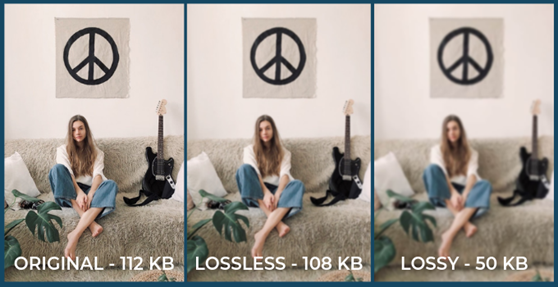
\includegraphics[scale=.7]{pic/compressiom.png}
    \caption[ความแตกต่างของการบีบอัดข้อมูล]{ความแตกต่างของการบีบอัดข้อมูล}
    \label{fig:compressiom}
  \end{center}
\end{figure}



\section{การส่งข้อมูลโดยใช้โปรโตคอลเอชทีทีพี (HyperText Transfer Protocol: HTTP) }
เป็นโปรโตคอลที่ใช้งานในด้านเว็บไซต์และในระบบอินเตอร์เน็ต สามารถสื่อสารกับข้ามแพลตฟอร์มมักจะนิยมใช้งาน HTTP 
เนื่องจากเป็นโปรโตคอลมาตรฐานที่มีมาให้ใช้งานในทุกภาษา และทุกอุปกรณ์ที่เชื่อมต่ออินเตอร์เน็ตได้ พื้นฐานของ HTTP มาจากโปรโตคอล (Transmission Control Protocol: TCP) 
ที่มีการใช้เพื่อรับ-ส่งข้อมูลในรูปแบบตามมาตรฐาน และใช้พอร์ต 80 เป็นค่าเริ่มต้น โดยผู้รับบริการ (HTTP Client) จะส่งข้อมูลผ่านคำสั่งการร้องขอแบบ POST 
เป็นคำสั่งที่ให้ส่งข้อมูลโดยแฝงข้อมูลไปกับเลขที่อยู่ไอพี (IP address) และใช้ร้องขอข้อมูลจากผู้ให้บริการ (HTTP Server) \cite{Http} ดังรูป

\begin{figure}[!ht]
  \begin{center}
    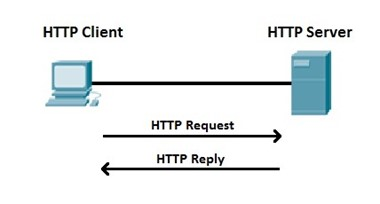
\includegraphics[scale=.8]{pic/http.jpg}
    \caption[โปรโตคอล HTTP]{โปรโตคอล HTTP}
    \label{fig:http}
  \end{center}
\end{figure}

\section{Raspberry Pi}
เครื่องคอมพิวเตอร์ขนาดเล็ก มีคุณสมบัติเด่น คือ ติดต่อ และความคุมอุปกรณ์อิเล็กทรอนิกส์ได้ โดยใน Raspberry Pi 
ได้รวมเอาซีพียู (CPU) หน่วยความจำ (Memory) และพอร์ต (Port) ซึ่งเป็นส่วนประกอบหลักสำคัญของระบบคอมพิวเตอร์เข้าไว้ด้วยกัน 
โดยทำการบรรจุเข้าไว้ในตัวถังเดียวกัน และสามารถเชื่อมต่ออินเทอร์เน็ตผ่านพอร์ตแลนหรือผ่านเครือข่ายไร้สาย \cite{PI} เช่น WiFi
	ในโครงงานนี้ได้เลือกใช้ Raspberry Pi มาเป็นอุปกรณ์ในการรับรูปภาพและค้นห้าใบหน้าในรูปภาพแบบเรียลไทม์ ส่งรูปภาพไปยังเซิร์ฟเวอร์ 
รอรับผลลัพธ์กลับมาแสดงผล ซึ่งใช้พลังงานต่ำ กินกระแสไม่เกิน 2A ในสภาวะการทำงานปกติ และสามารถเชื่อมต่ออินเทอร์เน็ตผ่านระบบไวไฟ (Wi-Fi) 
เพื่อในการรับส่งข้อมูลจากเซิร์ฟเวอร์


\section{Opensource Computer Vision (OpenCV)}
ไลบรารีโอเพ่นซอร์สที่นิยมสำหรับการประมวลผลภาพขั้นพื้นฐาน เช่น การเบลอภาพ การผสมภาพ การเพิ่มคุณภาพของภาพ 
เพิ่มคุณภาพของวิดีโอ การรู้จำวัตถุต่าง ๆ ในภาพ หรือ การตรวจจับใบหน้าหรือวัตถุต่าง ๆ ในภาพและวิดีโอได้ 
ปัจจุบัน (ปี 2022) OpenCV ได้พัฒนามาจนถึงรุ่นที่ 4 (Version 4) โดยในโครงงานนี้ได้เลือก OpenCV มาใช้ในการปรับแต่งรูป 
การตรวจจับใบหน้าแบบเรียลไทม์ และการระบุตัวตน \cite{OpenCV}

\section{Deep Learning}
ศาสตร์แขนงหนึ่งของการเรียนรู้ของเครื่อง (Machine Learning: ML) ทีเลียนแบบการทำงานของโครงข่ายประสาทของมนุษย์ (Neurons) 
โดยนำระบบโครงข่ายประสาท (Neural Network) มาซ้อนกันหลายชั้น (Layer)
และทำการเรียนรู้ข้อมูลตัวอย่าง ซึ่งข้อมูล ดังกล่าวจะถูกนำไปใช้ในการตรวจจับรูปแบบ (Pattern) หรือจัดหมวดหมู่ข้อมูล (Classify the Data)
ดังนั้นความสามารถของมันในอนาคตอาจจะเหนือมนุษย์ เนื่องจากสามารถเพิ่มพลังประมวลผลได้ไม่จำกัด 
ซึ่ง (Deep Learning: DL) คือโครงข่ายประสาทเทียม (Artificial Neural Network: ANN) ที่มีชั้นภายใน (Hidden layer) หลายชั้น 
เพื่อความสามารถในการคิดที่มากกว่าปกติ และสะท้อนสมองคนได้ดีขึ้น \cite{DEEP}
\\

\begin{figure}[!ht]
  \begin{center}
    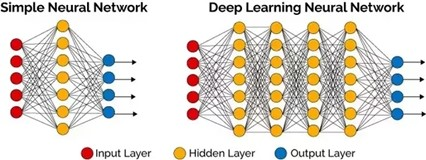
\includegraphics[scale=0.8]{pic/deep1.jpg}
    \caption[โครงสร้าง Deep Learning]{โครงสร้าง Deep Learning}
    \label{fig:deep1}
  \end{center}
\end{figure}

จะเห็นว่ามี 3 ส่วนคือ ชั้นรับข้อมูล (Input layer) ชั้นภายใน (Hidden layer) และชั้นแสดงผล (Output layer)
\begin{enumerate}
  \item ชั้นรับข้อมูล (Input layer) เป็นจุดเริ่มต้นของขั้นตอนการทำงานสำหรับ ANN จะทำหน้าที่ส่งข้อมูลไปยังแต่ละจุดต่อ (Node) ของชั้น (Layer)
  \item ชั้นภายใน (Hidden layer) เป็นส่วนที่ทำหน้าที่ส่งต่อข้อมูลไปยังชั้นแสดงผล (Output Layer) โดยแต่ละครั้งที่ข้อมูลการฝึกอบรม(Training Data) 
  ผ่านชั้น (Layer) นี้ไป แต่ละจุดต่อ (Node) จะค่อย ๆ ปรับน้ำหนัก (Weight) ให้เข้ากับข้อมูล (Data) มากขึ้นหรือถ้าอธิบายแบบเป็นทางการ 
  Hidden Layer จะคอยกักเก็บความซับซ้อนของชั้น (Layer) อื่น ๆ โดยการหาความสัมพันธ์ระหว่างคุณสมบัติ (Feature) ของข้อมูล (Data)
  \item ชั้นแสดงผล (Output layer) เป็นส่วนที่จะแสดงผล (Output) ซึ่งจำนวนจุดต่อ (Node) ในชั้นแสดงผล (Output layer) จะขึ้นอยู่กับจำนวนประเภท (Class) 
  ในข้อมูล (Data) อย่างเช่นจะสร้าง ANN เพื่อจำแนกหมากับแมว ก็ต้องมีจุดต่อแสดงผล (Output Node) 2 จุด และเมื่อใช้กับปัญหาการถดถอย (Regression Problems) ก็ต้องมี 1 จุดต่อ (Node) เท่านั้น 
  เพราะทำนาย (Predict) แค่ตัวเลข
\end{enumerate}
DL มีชั้นภายใน (Hidden layer) หลายชั้นทำให้มันสามารถคำนวณอะไรที่ซับซ้อนได้ และสามารถใช้เทคนิคต่าง ๆ ได้มากขึ้น และคิดอย่างเป็นขั้น เป็นตอนได้ดั่งรูป \\

\begin{figure}[!ht]
  \begin{center}
    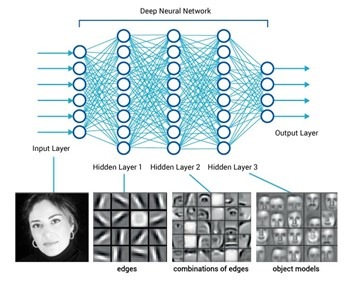
\includegraphics[scale=.9]{pic/deep2.jpg}
    \caption[Deep Learning ที่มีหลาย Hidden ayer]{Deep Learning ที่มีหลาย Hidden ayer}
    \label{fig:deep2}
  \end{center}
\end{figure}

\section{ส่วนต่อประสานกราฟิกกับผู้ใช้ (Graphical User Interface: GUI)}
การติดต่อกับผู้ใช้โดยใช้ภาพสัญลักษณ์ เป็นการออกแบบส่วนของโปรแกรมคอมพิวเตอร์ให้มีการโต้ตอบกับผู้ใช้ โดยการใช้ สัญรูป (Icon) รูปภาพ และสัญลักษณ์อื่น 
เพื่อแทนลักษณะต่าง ๆ ของโปรแกรม แทนที่ผู้ใช้จะพิมพ์คำสั่งต่าง ๆ ในการทำงาน ช่วยทำให้ผู้ใช้งานสามารถทำงานได้ง่าย และรวดเร็วขึ้น ไม่ต้องจดจำคำสั่งต่าง ๆ 
ของโปรแกรม เป็นวิธีการให้ความสะดวกแก่ผู้ใช้คอมพิวเตอร์ ให้ติดต่อสื่อสารกับระบบโดยผ่านทางภาพ เช่น ใช้เมาส์กดเลือกสัญรูป (Icon) แทนการพิมพ์คำสั่งดังแต่ก่อน 
โดยเฉพาะในบางโปรแกรมที่มีคำสั่งจำนวนมาก ซึ่งทำให้ไม่ต้องพิมพ์คำสั่งต่าง ๆ ทางแป้นพิมพ์ ช่วยทำให้เกิดความรวดเร็วในการทำงาน 
และไม่ต้องเสียเวลาในการเรียนรู้และจดจำคำสั่งที่ต้องการมากนัก เพียงดูจากไอคอนที่ปรากฏในโปรแกรมก็สามารถใช้งานได้ทันที \cite{GUI}

\section{Tkinter}
Tkinter หรือ Tk เป็นมอดูลที่พัฒนามาจาก Tk GUI Toolkit ซึ่งทางานอยู่บนระบบปฏิบัติการยูนิกซ์มาก่อนไพธอน (Python) ได้เลือกมอดูลนี้ในการพัฒนากราฟิกบนไพธอน (Python) เป็นหลัก
ประกอบไปด้วย 3 ส่วนที่สำคัญคือ วิดเจ็ต (Widgets) การจัดการรูปทรงเรขาคณิตให้กับวิดเจ็ต (Geometry management) และ การจัดการกับเหตุการณ์ต่าง ๆ (Event Handling) \cite{Tkinter} ซึ่งมีรายละเอียดดังนี้
\begin{enumerate}
  \item วิดเจ็ต (Widgets) คือ สิ่งต่าง ๆ หรือเรียกว่า อ๊อปเจ็กต์ (Object) ที่ปรากฏอยู่บนจอภาพ เช่น ปุ่ม (Button) ตัวหนังสือ (Label) เฟรม (Frame) กล่องเลือก (Checkbox) 
  วิวต้นไม้ (Tree views) แถบเลื่อน (Scrollbars) และกล่องข้อความ (Text areas) เป็นต้น
  \item การจัดการรูปทรงเรขาคณิตให้กับวิดเจ็ต (Geometry management) คือ การวางวิดเจ็ต (Widgets) ลงบนเฟรม (Frame) นั้นจะต้องกำหนดตำแหน่งในการวาง 
  โดยอาศัยศาสตร์ทางด้านเรขาคณิตเข้าช่วย เพื่อให้วิดเจ็ต (Widgets) ที่จะวางอยู่ในตำแหน่งที่เหมาะสม ซึ่งไพธอน (Python) มี 3 เมธอดในการจัดการเกี่ยวกับเรขาคณิตของวิดเจ็ต (Widgets) 
  ประกอบไปด้วยเมธอด pack(), grid() และ place()
  \item การจัดการกับเหตุการณ์ต่าง ๆ (Event Handling)  คือ เหตุการณ์ต่าง ๆ ที่ผู้ใช้งานกระทำกับวิดเจ็ต (Widgets) บน GUI เช่น การกดปุ่ม การกดปุ่มใด ๆ บนแป้นพิมพ์ 
  การเคลื่อนเมาส์ การปรับขนาดของหน้าต่างวินโดวส์ เป็นต้น เหตุการณ์ต่าง ๆ เหล่านี้จะถูกจัดการโดย Tk ซึ่งเรียกว่าวนรอบเหตุการณ์ (Event loop) โดยจะทำงานร่วมกับระบบปฏิบัติการโดยตรง 
  เช่น เมื่อเคลื่อนเมาส์ไปยังปุ่มจะส่งผลให้ปุ่มดังกล่าวจะเปลี่ยนสี และเมื่อเคลื่อนเมาส์ออกจากปุ่มจะทำให้สีของปุ่มกลับไปเป็นสีเดิม เป็นต้น
\end{enumerate}

\section{OpenFace (Open-source Face Recognition)}
มอดูลที่ใช้ในการระบุตัวตนด้วยรูปภาพใบหน้าของมนุษย์ที่ทำงานร่ามกับ DNN และเป็นมอดูลแบบโอเพนซอร์ส \cite{amos2016openface} โดยมีหลักการทำงาน ดังนี้
\begin{enumerate}
  \item ตรวจจับใบหน้าด้วยโมเดลที่ผ่านการฝึกอบรมล่วงหน้า
  \item แปลงใบหน้าสำหรับโครงข่ายประสาทเทียม ทำงานร่วมกับ OpenCV เพื่อทำให้ดวงตา และริมฝีปากล่างปรากฏในตำแหน่งเดียวกัน และสัมพันในแต่ละภาพ
  \item ใช้โครงข่ายประสาทเทียมเชิงลึก (DNN) เพื่อแสดงหรือฝังใบหน้าบนหน่วยไฮเปอร์สเฟียร์ 128 มิติ การฝังเป็นการแสดงความแตกต่างสำหรับใบหน้าของใครก็ตาม 
  ซึ่งแตกต่างจากใบหน้าอื่น ๆ การฝังนี้ทำให้เห็นคุณสมบัติที่ต่างกันมากขึ้นระหว่างใบหน้าสองใบหน้า ซึ่งทำมให้ทราบว่าใบหน้านั้นไม่น่าจะใช่คนคนเดียวกันหรือเป็นคนคนเดียวกัน 
  คุณสมบัตินี้ทำให้การจัดกลุ่ม การตรวจจับความคล้ายคลึงกัน และการจัดหมวดหมู่ทำได้ง่ายกว่าเทคนิคการจดจำใบหน้าอื่น ๆ โดยที่ระยะห่างแบบยุคลิดระหว่างคุณลักษณะต่าง ๆ 
  ไม่มีความหมาย
  \item ใช้เทคนิคการจัดกลุ่ม หรือการจัดหมวดหมู่ที่สนใจกับคุณสมบัติต่าง ๆ เพื่อทำงานการจดจำของใบหน้าบุคคล 
\end{enumerate}  


\begin{figure}[!ht]
  \begin{center}
    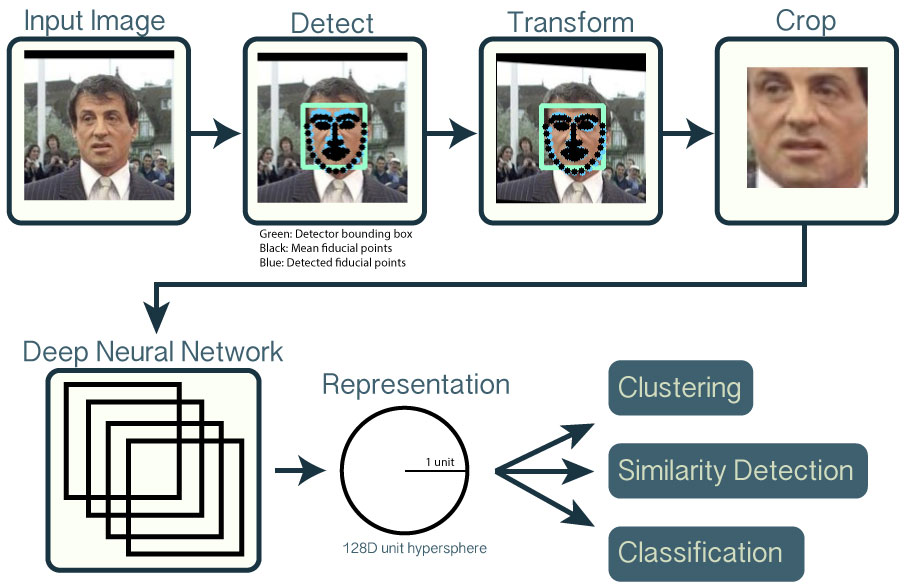
\includegraphics[scale=.25]{pic/openface.jpg}
    \caption[การทำงานของ OpenFace]{การทำงานของ OpenFace}
    \label{fig:opemface}
  \end{center}
\end{figure}



\section{\ifenglish%
\ifcpe CPE \else ISNE \fi knowledge used, applied, or integrated in this project
\else%
ความรู้ตามหลักสูตรซึ่งถูกนำมาใช้หรือบูรณาการในโครงงาน
\fi
}

\subsection{Logic and Digital Circuits และ Microprocessor and Interfacing}

ใช้ความรู้จากสองวิชานี้ในการออกแบบระบบการทำงานของอุปกรณ์ของโครงสร้างชิ้นงานใน
แต่ละส่วน และการเขียนโปรแกรมเพื่อควบคุมการทำงานของอุปกรณ์

\subsection{Digital Image Processing}

ใช้ความรู้จากวิชานี้ในการออกแบบการบีบอัดรูปภาพ การจัดเก็บรูปภาพ การทำให้รูปภาพมีคุณภาพที่ดีขึ้นเพื่อให้ความแม่นยำของการทำนายสูงขึ้น

\subsection{Deep Learning}
เรียนรู้โครงสร้าง และการทำงานของ Neuron Network เพื่อหาโมเดลการรีะบุตัวตนที่เหมาะสมกับงาน

\subsection{CPE Lab}
ใช้ในการทำ Web service และออกแบบ GUI

\section{\ifenglish%
Extracurricular knowledge used, applied, or integrated in this project
\else%
ความรู้นอกหลักสูตรซึ่งถูกนำมาใช้หรือบูรณาการในโครงงาน
\fi
}
\begin{itemize}
  \item การใช้งาน Raspbian OS ของ Raspberry Pi
  \item การตั้งค่ากล้องให้กับ Raspberry Pi และระบบ GPIO ของ Raspberry Pi เพื่อติดตั้งชุดระบายความร้อน
\end{itemize}


% \subsubsection{Subsubsection 1 heading goes here}
% Subsubsection 1 text

% \subsubsection{Subsubsection 2 heading goes here}
% Subsubsection 2 text

% \section{Third section}
% Section 3 text. The dielectric constant\index{dielectric constant}
% at the air-metal interface determines
% the resonance shift\index{resonance shift} as absorption or capture occurs
% is shown in Equation~\eqref{eq:dielectric}:

% \begin{equation}\label{eq:dielectric}
% k_1=\frac{\omega}{c({1/\varepsilon_m + 1/\varepsilon_i})^{1/2}}=k_2=\frac{\omega
% \sin(\theta)\varepsilon_\mathit{air}^{1/2}}{c}
% \end{equation}

% \noindent
% where $\omega$ is the frequency of the plasmon, $c$ is the speed of
% light, $\varepsilon_m$ is the dielectric constant of the metal,
% $\varepsilon_i$ is the dielectric constant of neighboring insulator,
% and $\varepsilon_\mathit{air}$ is the dielectric constant of air.

% \section{About using figures in your report}

% % define a command that produces some filler text, the lorem ipsum.
% \newcommand{\loremipsum}{
%   \textit{Lorem ipsum dolor sit amet, consectetur adipisicing elit, sed do
%   eiusmod tempor incididunt ut labore et dolore magna aliqua. Ut enim ad
%   minim veniam, quis nostrud exercitation ullamco laboris nisi ut
%   aliquip ex ea commodo consequat. Duis aute irure dolor in
%   reprehenderit in voluptate velit esse cillum dolore eu fugiat nulla
%   pariatur. Excepteur sint occaecat cupidatat non proident, sunt in
%   culpa qui officia deserunt mollit anim id est laborum.}\par}

% \begin{figure}
%   \centering

%   \fbox{
%      \parbox{.6\textwidth}{\loremipsum}
%   }

%   % To include an image in the figure, say myimage.pdf, you could use
%   % the following code. Look up the documentation for the package
%   % graphicx for more information.
%   % \includegraphics[width=\textwidth]{myimage}

%   \caption[Sample figure]{This figure is a sample containing \gls{lorem ipsum},
%   showing you how you can include figures and glossary in your report.
%   You can specify a shorter caption that will appear in the List of Figures.}
%   \label{fig:sample-figure}
% \end{figure}

% Using \verb.\label. and \verb.\ref. commands allows us to refer to
% figures easily. If we can refer to Figures
% \ref{fig:overview} and \ref{fig:sample-figure} by name in the {\LaTeX}
% source code, then we will not need to update the code that refers to it
% even if the placement or ordering of the figures changes.

% \loremipsum\loremipsum

% % This code demonstrates how to get a landscape table or figure. It
% % uses the package lscape to turn everything but the page number into
% % landscape orientation. Everything should be included within an
% % \afterpage{ .... } to avoid causing a page break too early.
% \afterpage{
%   \begin{landscape}
%   \begin{table}
%     \caption{Sample landscape table}
%     \label{tab:sample-table}

%     \centering

%     \begin{tabular}{c||c|c}
%         Year & A & B \\
%         \hline\hline
%         1989 & 12 & 23 \\
%         1990 & 4 & 9 \\
%         1991 & 3 & 6 \\
%     \end{tabular}
%   \end{table}
%   \end{landscape}
% }

% \loremipsum\loremipsum\loremipsum

% \section{Overfull hbox}

% When the \verb.semifinal. option is passed to the \verb.cpecmu. document class,
% any line that is longer than the line width, i.e., an overfull hbox, will be
% highlighted with a black solid rule:
% \begin{center}
% \begin{minipage}{2em}
% juxtaposition
% \end{minipage}
% \end{center}

